\begin{itemize}
    \item Drei Anwendungen, jeweils eine aus den Bereichen Messwerte, Nowcasting, Forecasting
    \item Messwerte: Daten Medizinmesswerte
    \item Nowcasting: Covid-Nowcasting-Hub
    \begin{itemize}
        \item Daten sind schon aufbereitet
        \item Vergleich zwischen Nowcastern möglich
        \item Noch zu klären: Wie wird $\xdiff$ gewählt?
    \end{itemize}
    \item Forecasting: Pandemie-/Epidemievorhersage, Medikamentenbedarf
\end{itemize}

\subsection{Covid nowcasting}

Data from Covid-Nowcasting-Hub

Besprechen

\begin{itemize}
    \item Was ist x-calligrafisch? aktuell betrachteter Nowcast oder "bester" Nowcast? Aktuell betrachteter Nowcast (keine "Auswahl" nötig mit Maß, Trainingsdatensatz, Rolling Fit, ...)
    \item Welche Lags werden betrachtet? Tage, Woche(n)
    \item Wie geht man mit missing values um? Vor allem auch für missing values für manche issued-times, wenn es aber andere issed-times gibt, für die Werte vorliegen?
    \begin{itemize}
        \item Imputation (2. Wahl)
        \item Nachgereichte Werte mit ursprünglichen Daten (1. Wahl)
        \item Nachgereichte Werte mit späteren Daten $\rightarrow$ nicht benutzen
    \end{itemize}
\end{itemize}

\subsection{Forecasting emergeny department arrivals}

\textcite{Rostami-Tabar2023}

Paper setup:

\begin{itemize}
    \item (Probabilistic) forecast of the hourly number of arrivals in large emergency department (take expectation as point forecast)
    \item Forecasts are produced 48 hours ahead on a 12-hour-rolling basis; background: \enquote{It enables planners to match ED staff to the number of arrivals, redeploy staff, and reconfigure units.}
    \item training data: 2014-04-01 to 2018-2-28
    \item evaluation from 2018-03-01 to 2019-02-28
    \item Evaluation in Paper through RMSE; Pinball Loss and PIT-histograms
    \item consider several lags:
    \begin{itemize}
        \item 72-hours-lag: Is the forecast showing the correct change compared to the most recent observation (problem: strong weekly structure (i.e., Monday and Saturday highest) makes it easy to predict right direction)
        \item 7-days-lag: Correct trend compared to the last shift of same hour and day $\rightarrow$ change policies compared to that
        \item Take first issued forecast for every target time
    \end{itemize}
\end{itemize}

\begin{table}
\centering
\begin{tabular}{llll}
\toprule
 & trend acc lag 3d & trend acc lag 7d & rmse \\
\midrule
Benchmark-1 & 0.7867 & 0.7556 & 10.0654 \\
Benchmark-2 & 0.7847 & 0.7615 & 9.2462 \\
Poisson-1 & 0.7876 & 0.7661 & 9.1639 \\
Poisson-2 & 0.7886 & 0.7655 & 8.8838 \\
NOtr-1 & 0.7829 & 0.7609 & 9.4132 \\
NOtr-2 & 0.7829 & 0.7609 & 9.4132 \\
GBM-2 & 0.7697 & 0.7413 & 11.6628 \\
Ttr-2 & 0.7857 & 0.7651 & 9.3944 \\
NBI-2 & 0.7895 & 0.7656 & 8.8829 \\
qreg-1 & 0.7501 & 0.7291 & 13.3367 \\
Poisson-2-I & 0.7834 & 0.7615 & 9.4579 \\
tbats & 0.6906 & 0.6659 & 12.9049 \\
ADAM-iETSX & 0.6794 & 0.6633 & 28.0003 \\
ETS & 0.6561 & 0.6471 & 29.3577 \\
Regression-Poisson & 0.6930 & 0.6742 & 21.1623 \\
Prophet & 0.6864 & 0.6724 & 13.0785 \\
\bottomrule
\end{tabular}

\caption{Accuracies (without exclusion area) and RMSE for the considered models in \textcite{Rostami-Tabar2023}}	
\end{table}

\begin{figure}
	\centering
	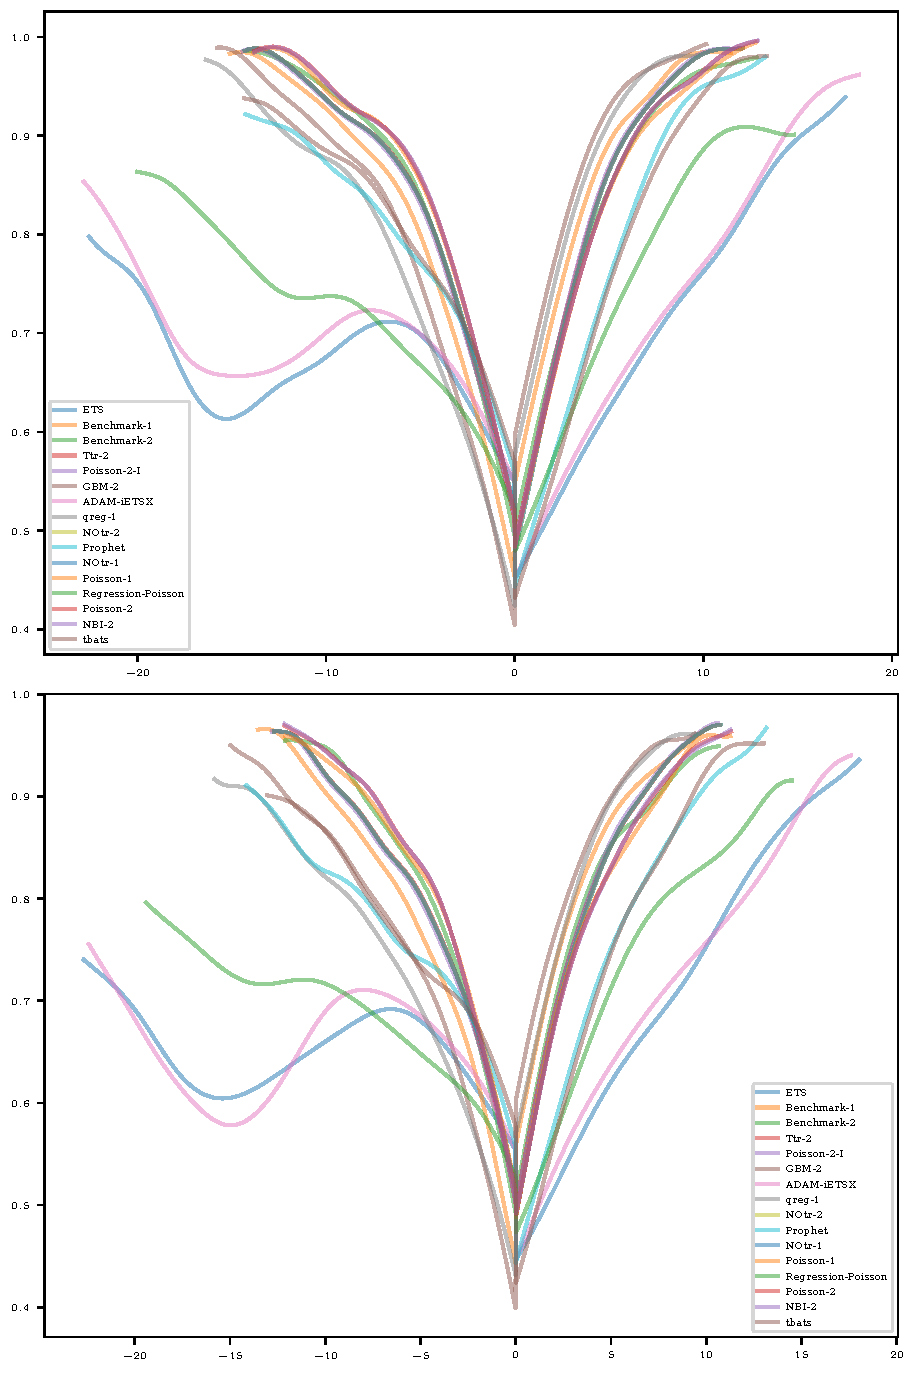
\includegraphics{plots/ed_arrival/CondProbs.pdf}
\end{figure}